
\section{Optimierung des DSP}
Nach dem in dem vorherigen Kapitel die Optimierung des Musikklassifikators aufm dem ARM Cortex-A8 beschrieben wurde, behandelt dieses Kapitel die Optimierung der Extraktionsphase auf dem C674x DSP von Texas Instruments.\\
Als erstes muss der C++-Referenzcode in C-Code �bersetzt werden, da der C674x nur diesen ausf�hren kann. Anschlie�end werden durch eine Laufzeitmessung die Laufzeitantiele der einzelnen Feature-Berechnungen ermittelt (siehe \textbf{Abbildung \ref{fig:startdsp}}).
%
\begin{figure}[h]
	\centering
		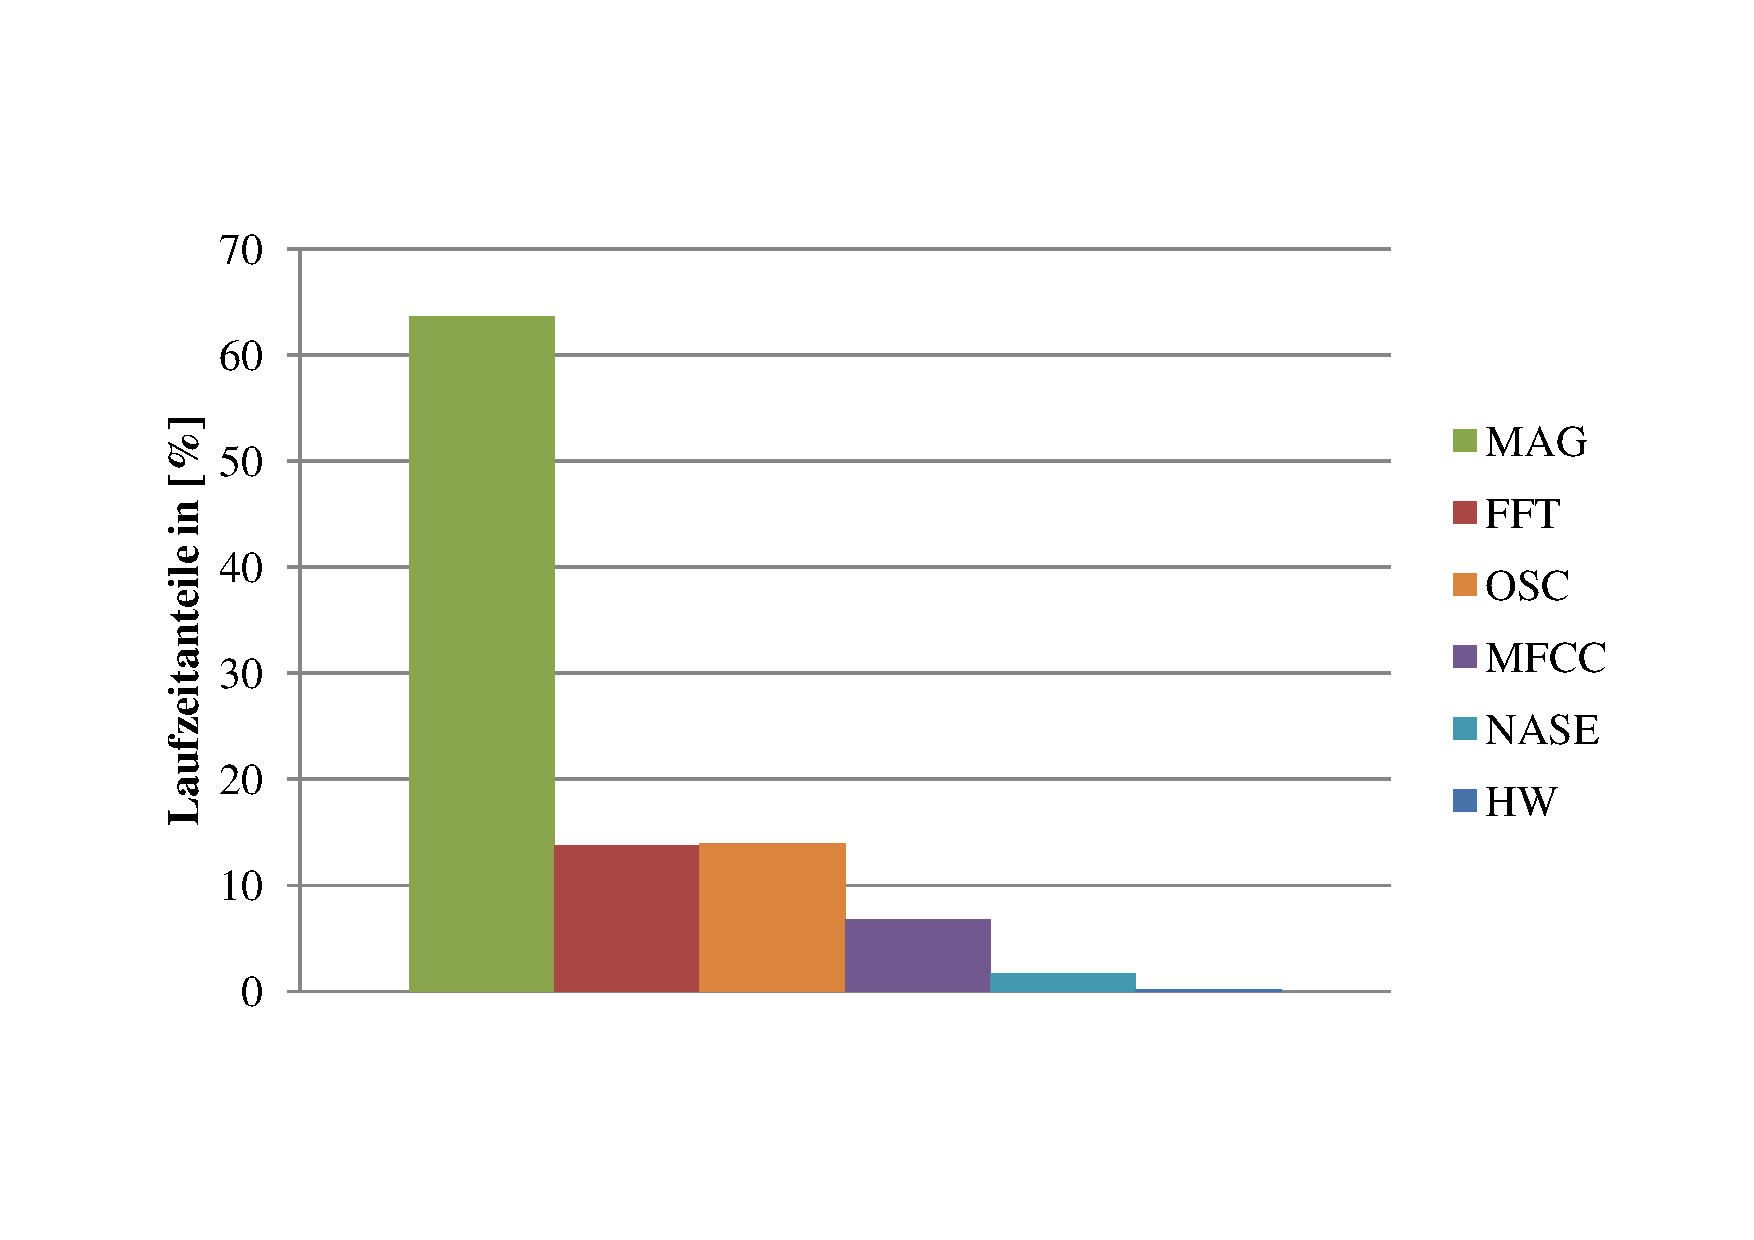
\includegraphics[width=1\textwidth]{../Pictures/startdsp.pdf}
	\caption{Laufzeitanteile der einzelnen Features}
	\label{fig:startdsp}
\end{figure} 
%
Wie man der Abbildung entnehmen kann f�llt der gr��te Anteil mit �ber 60\% der Magnitude of Spectrum zu, aber auch FFT und Octave Spectral Contrast mit je 14\% sind nicht zu vernachl�ssigen.\\
Ein Detailprofiling der Magnitude of Spectrum ergibt, dass Division und Wurzelberechnung zusammen knapp 98\% der Laufzeit ausmachen, das hei�t, dass eine Optimierung in Richtung der Rechenfunktionen geschehen sollte.

\subsection{Optimierung der Rechenfunktionen mit MATHLIB}\label{sec:mathlib}
Da wie bereits erw�hnt, die Rechenfunktionen bei zum Beispiel der Magnitude of Spectrum als Bottlenecks identifiziert wurden und wie in \textbf{Kapitel \ref{subsubsec:optbib}} erw�hnt eine Bibliothek (MATHLIB) existiert, in der genau diese Rechenoperationen optimiert wurden, werden alle problematischen Funktionen durch ihre optimierten Varianten ersetzt. Wie ebenfalls in dem Kapitel erw�hnt, existieren f�r alle in MATHLIB implementierten Operationen auch Varianten, die auf Vektoren von Eingangswerten arbeiten k�nnen. Daher wird als erstes versucht, soweit es m�glich ist, Operationen wie zum Beispiel Divisionen, Wurzelberechnungen oder Logarithmusfunktionen durch diese Vektoroperationen zu ersetzten. Sollte eine Ersetzung durch Vektoroperationen nicht m�glich sein, werden Einzelaufrufe durch die optimierten Varianten der MATHLIB ersetzt.\\
Diese Ersetzung wird Beispielhaft f�r Magnitude of Spectrum in \textbf{Listing \ref{code:aoscc}} und \textbf{Listing \ref{code:aoscm}} gezeigt.
\newpage
\begin{lstlisting}[caption=Referenzcode von Magnitude of Spectrum, label=code:aoscc]
	A[k] = sqrt(X[k] * X[k] + Y[k] * Y[k]) / G;
\end{lstlisting}

\begin{lstlisting}[caption=Magnitude of Spectrum mit MATHLIB, label=code:aoscm]
	for (k = 0; k < G; ++k) {
		tmp1 = X[k] * X[k];
		tmp2 = Y[k] * Y[k];
		A[k] = (tmp1 + tmp2); //(X[k] * X[k] + Y[k] * Y[k]);
	}
	
	sqrtsp_v(A, A, G);

	divsp_v(A, pG, A, G);
\end{lstlisting}

Die Akkumulation innerhalb der Wurzelberechnung wurde zus�tzlich f�r eine bessere Ausf�hrung durch SPLOOP getrennt.\\
Eine Optimierung mit MATHLIB wurde bei folgenden Algorithmen durchgef�hrt:

\begin{itemize}
\item Magnitude of Spectrum
\item MFCC
\item Low Energy
\item Normalized Audio Spectrum Envelope
\item Octave Spectral Contrast
\item Root Mean Square
\item Spectral Centroid
\item Spectral Crest Factor
\item Spectral Flux
\item Sub-band Energy Ratio
\end{itemize}

Abschlie�end wird nach der Optimierung mit MATHLIB eine weitere Laufzeitmessung durchgef�hrt. Diese soll zwei Dinge zeigen:

\begin{enumerate}
\item ist Magnitude of Spectrum immer noch der gr��te Bottleneck oder
\item haben sich neue Bottlenecks aufgetan
\end{enumerate}
%
\begin{figure}[h]
	\centering
		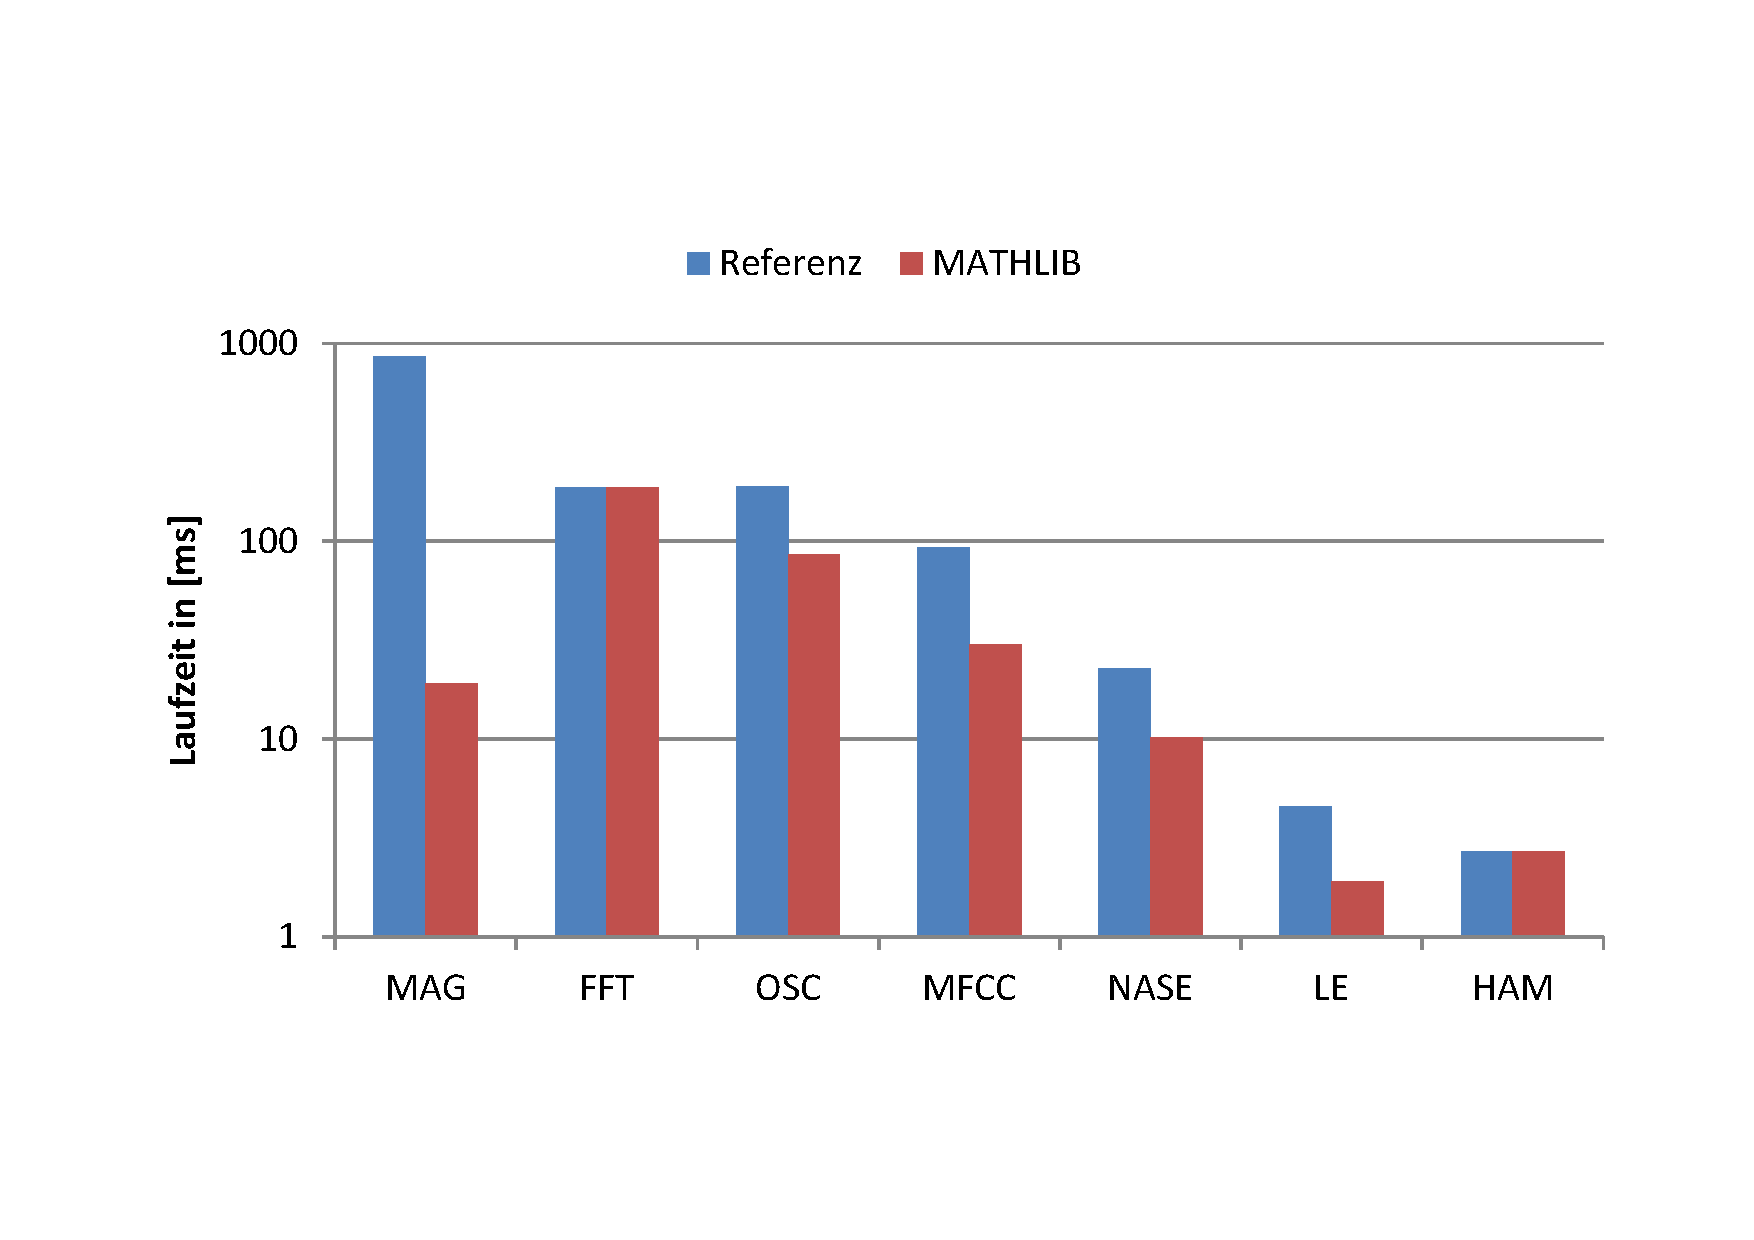
\includegraphics[width=1\textwidth]{../Pictures/dsp2.pdf}
	\caption{Laufzeitmessung nach der Optimierung durch MATHLIB}
	\label{fig:dsp2}
\end{figure} 
%
\textbf{Abbildung \ref{fig:dsp2}} zeigt die angesprochene Laufzeitmessung. Wie man dort erkennen kann, ist Magnitude of Spectrum nicht mehr der gr��te Bottleneck, jetzt zeigt sich, dass die FFT-Berechnung zum gr��ten Bottleneck geworden ist, also wird in diese Richtung weiter optimiert.

\subsection{Optimierung der FFT mit DSPLIB}\label{sec:dsplib}
Wie ebenfalls in \textbf{Kapitel \ref{subsubsec:optbib}} erw�hnt, wird von Texas Instruments auch eine optimierte Bibliothek bereitgestellt, in der eine FFT-Implementierung vorhanden ist. Durch diesen Umstand macht es Sinn diese f�r die Optimierung der FFT-Berechnung zu verwenden.\\
Bei der FFT aus der DSPLIB handelt es sich um eine Complex2Complex-Mixedradix-FFT. Diese C2C-FFT l�sst sich aber nach der in \cite{rfft} beschriebenen Methode in eine Real2Complex-FFT umwandeln.\\
Die Einbindung der DSPLIB-FFT geschieht ebenfalls auf die in \cite{rfft} beschriebene Weise. Des weiteren wurde die �bergabe zwischen FFT und MAG ge�ndert, so dass ncith wie vorher je ein Signal f�r Real- und Imagin�rteil �bergeben werden, sondern ein einzelnes Signal in dem Real- und zugeh�riger Imagin�rteil hintereinander stehen. \\
Auch nach der Optimierung der FFT durch die Einbindung der DSPLIB wird wieder eine Laufzeitmessung durchgef�hrt um eventuell weitere Bottlenecks zu identifizieren.\\
%
\begin{figure}[h]
	\centering
		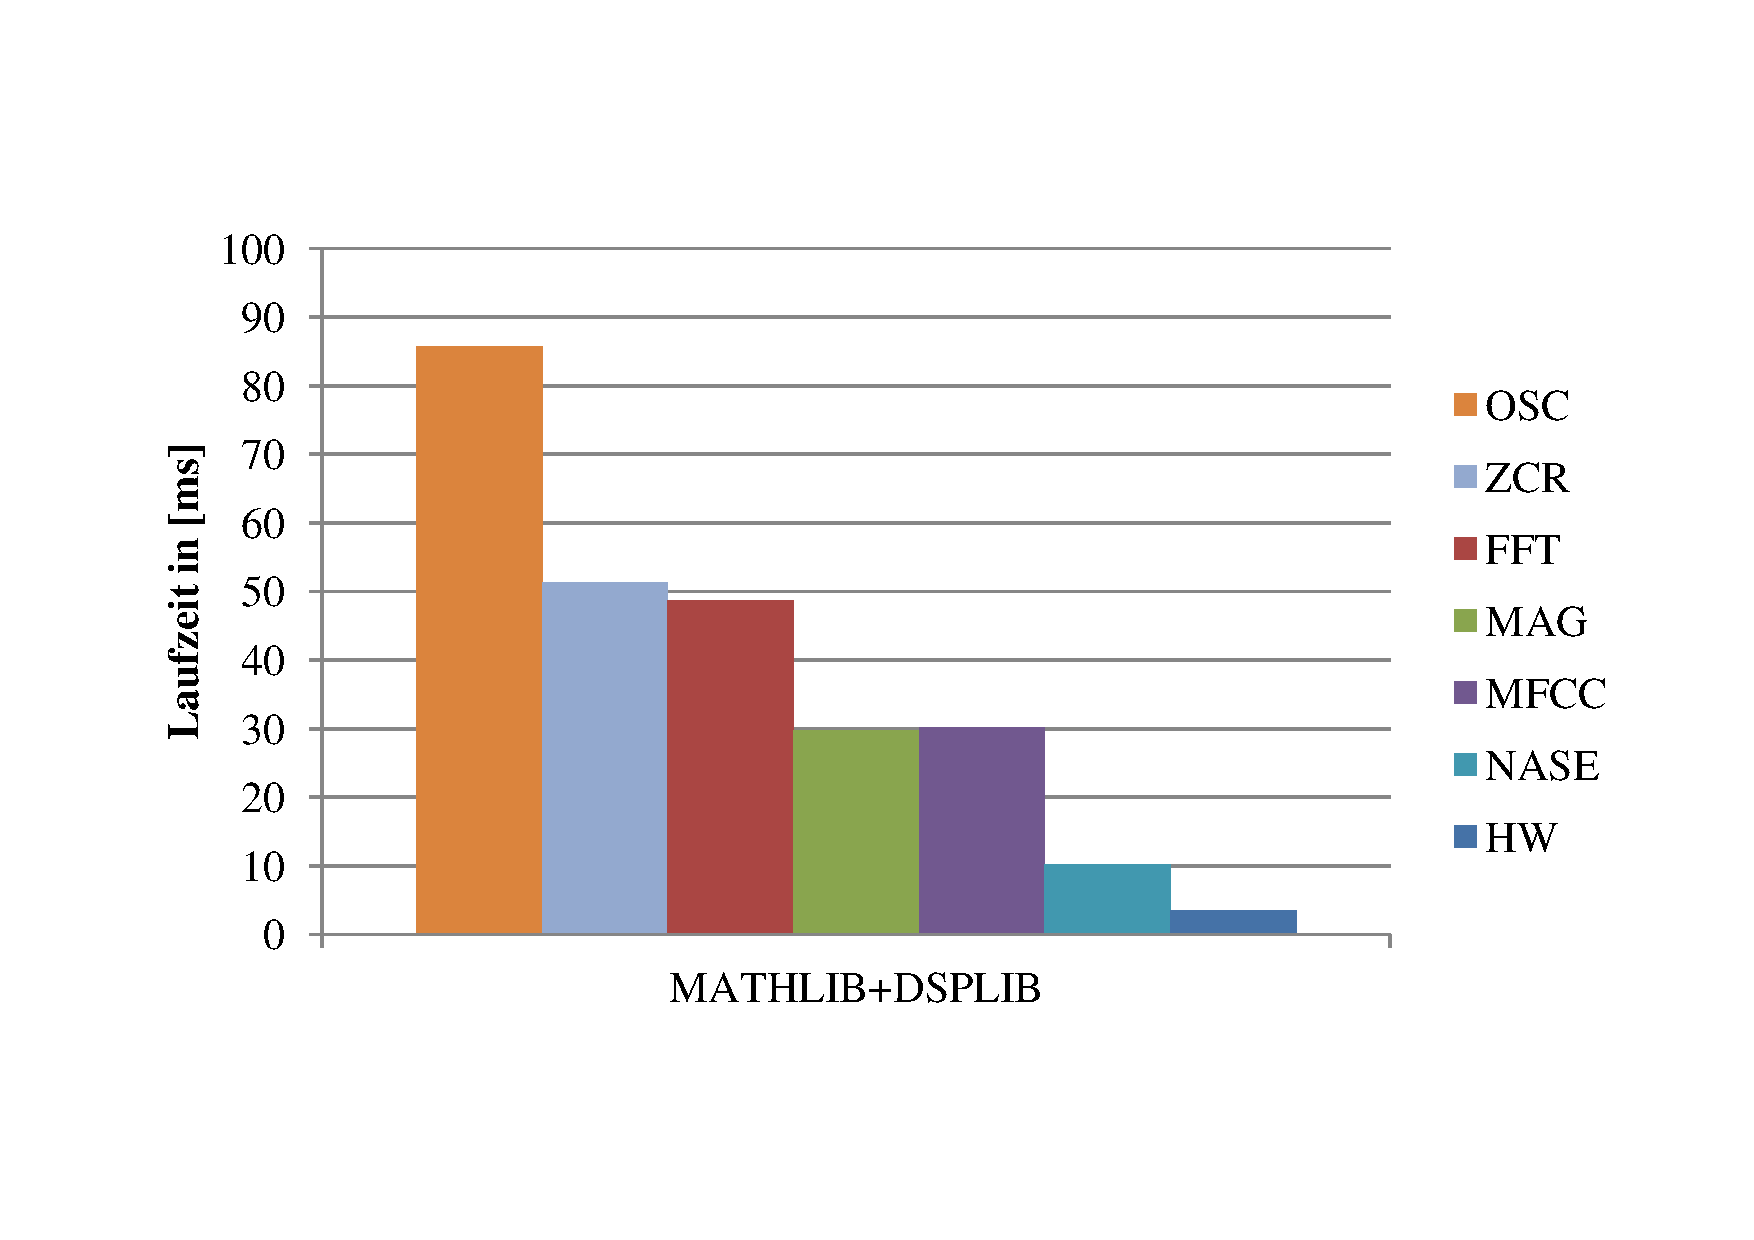
\includegraphics[width=1\textwidth]{../Pictures/dsp3.pdf}
	\caption{Laufzeitmessung nach der Optimierung durch MATHLIB und DSPLIB}
	\label{fig:dsp3}
\end{figure} 
%
\textbf{Abbildung \ref{fig:dsp3}} zeigt das Ergebnis der erw�hnten Laufzeitmessung, die Features aus FeatureSet 2 wurden um die Zero Crossing Rate aus FeatureSet 3 erg�nzt, da diese nach der FFT-Optimierung langsamer als die FFT ist.\\
Nach dieser Messung ergeben sich zwei neue Bottlenecks, Octave Spectral Contrast und Zero Crossing Rate. Bei OSC nimmt mit 55\% die Sortierung den gr��ten Anteil der Laufzeit ein, auch bei der DSP-Implementierung soll keine Optimierung in diese Richtung vorgenommen werden.

\subsection{Optimierung f�r SPLOOP}\label{sec:compiler} 
Ein Blick in den Assemblercode der Zero Crossing Rate zeigt, dass f�r die Schleife keine SPLOOP-Optimierung vom Compiler durchgef�hrt wurde. Dieses l�sst sich aber durch eine einfache Codeumstellung l�sen. \textbf{Listing \ref{code:zcrc}} zeigt den Referenzcode der Zero Crossing Rate und \textbf{Listing \ref{code:zcrs}} den umgestellen Code.

\begin{lstlisting}[caption=Referenzcode der Schleife der Zero Crossing Rate, label=code:zcrc]
	for (n = 0; n < zinfo.N - 1; ++n) {
		zero_crossings += ABS(SGN(signal[n])-SGN(signal[n+1]));
	}
\end{lstlisting}

\begin{lstlisting}[caption=F�r SPLOOP umgestellter Code der Schleife der Zero Crossing Rate, label=code:zcrs]
	for (n = 0; n < zinfo.N - 1; ++n) {
		tsgn1 = SGN(signal[n]);

		tsgn2 = SGN(signal[n+1]);

		tsub = tsgn1 - tsgn2;

		tabs = ABS(tsub);

		zero_crossings += tabs;
	}
\end{lstlisting}

\subsection{Zwischenevaluation der DSP-Optimierung}